\chapter{MC (Monte Carlo) Samples}
\label{sec:MCSamples}

In order to analyze the data we use the computer-generated data samples using the software that simulates the physical processes that happen in the detector. The process consists of several stages:
\begin{enumerate}
\item The simulation of the $pp$ collision, which involves the birth and the decay of high-energy particles (done by the MC generators, see sec.~\ref{sec:MC_gen})
\item The simulation of interactions between the high-energy particles and the substance of the detector (done by the Geant4 software, see sec.~\ref{sec:MC_sim_rec})
\item The simulation of the detector response based on the amount of deposited energy in different parts of the detectors (done by the ATLAS software)
\item The reconstruction process runs the same way as for the genuine data samples
\end{enumerate}
The simulation process takes lots of time, with the most time-consuming process being the simulation of the particles passing through the detector, or even more precise, through the EM-calorimeters, as the calorimeters consist of the very dense materials (e.g. lead and liquid argon) and hence the incoming high-energy particles produce the large showers with the tens of thousands of lower-energy particles. There are several technics used to speed up the process, but most of them produces the different result from the full simulation, which makes them unusable for many types of analysis (including \Zee). The only technology which gives the result close enough to the full simulation to be enabled for all analysis samples by default is the Frozen Showers, which will be fully described in sec.~\ref{sec:MC_FS}.

\section{MC generators used in ATLAS experiment}
\label{sec:MC_gen}

1. General physiscs (NLO, LO, PS, QED radiation ... ) 

\subsection{signal}
2. MC tuning and which one we use
3. What we use

MC@NLO+herwig PowHeg+herwig/pythia

photos for QED

CT10 PDF

\subsection{BG}
4. BG MCs (7 of them)

\section{MC production chain}
\label{sec:MC_sim_rec}

The output of the MC generators consists of the set of the final-state particles, which in turn are passed to the ATLAS MC production chain. This chain consist of three main stages, namely: the simulation, digitization and the reconstruction.

Although the whole process of the production of the MC samples can be considered as "simulation", in this context "the simulation process" refers to the particular stage of the whole production chain: the simulation of the propagation of the high-energy particles through the matter of the detector. It is done using the Geant4 software and the highly-accurate 3D model of the detector. The simulation in Geant4 is done as a discrete step-by-step process, with the length of the step being calculated dynamically for each particle, based on particle energy and the physical processes that happen to that particle. Because of that the simulation of the particles in vacuum takes much less time than in heavy matter. That is the reason why the majority of the simulation time is spent in calorimeters: they are built of the densest material there is in explicit purpose to stop as many particles as possible.

The output of the simulation stage is "hits", the 4D vertexes of energy deposits in sensitive areas of the detectors. The next stage is to simulate the work of the detector itself, or to convert the energy deposits into detector response, which are usually voltages on the read-out channels. This process is called "digitization", because it's output is "digits" which the read-out channels provide. During this stage all features of the detector logic are simulated (e.g. electric noises or channel-dependent variations). This is done by the internal ATLAS digitization software, and because it requires an intimate knowledge of every particular sub-detector, parts of it are maintained by separate groups related to the respective sub-detectors.

The last step in the production chain is the same for both MC and genuine data samples, as the digitization process aims to provide the same data as we get from the detector during production runs. During this step the responses from the detector are reconstructed into physical particles, which is done in two steps. First step is more on the technical side, during which the response from the trackers is reconstructed into tracks and the response from the calorimeters is reconstructed into clusters. The second stage is physical and depends on the analysis. During this stage the tracks and clusters are combined in the physical particles. The flavors of this stage of reconstruction include e/gamma, jet/EtMiss/tau, b tagging and muon. $\Zee$ analysis uses the first: e/gamma flavored reconstruction. This process is done using the internal ATLAS reconstruction software.

The result of the reconstruction is the data stored in the special format called AOD (Analysis Data Object), which is also developed internally by ATLAS. AODs can be read by the ATLAS analysis framework, which gives easy access to all reconstructed objects.

\begin{figure}[htb]
\center{

\includegraphics[width=1.0\textwidth]{figures/blank.eps}
\caption{Diagram of the ATLAS MC production chain}
\label{fig:MC_gen}}
\end{figure}

\subsection{Frozen Showers}
\label{sec:MC_FS}
The frozen showers system (FS) is a system that is designed to speed up the geant4 simulation process inside the EM calorimeters. The main principle of FS is to substitute the low-energy particles with the EM-showers, which are pre-simulated and stored in the libraries. These libraries must be generated in advance for each calorimeter and for each type of particles which is needed to be parameterized during the production simulation. The generation process consists mostly of the simulating of the low-energy particles and saving the information about every energy deposition this particle made. The array of these deposits or "hits" passes through several post-processing procedures in order to reduce it's size, and becomes a "shower".

\begin{figure}[htb]
\center{

\includegraphics[width=1.0\textwidth]{figures/blank.eps}
\caption{Diagram showing the shower substitution}
\label{fig:MC_FS_idea}}
\end{figure}

The generation of the shower library is thus a preparatory procedure, which needs to be done every time when something is changed in the geant4 simulation process. The examples are the change of the geant4 version used, or the change in the detector geometry. Usually these changes applied between the MC campaigns, which means that the new set of libraries needs to be generated for each campaign. In order to improve results of FS-enabled simulation the libraries are then tuned: the shape and the energy response of the stored showers are slightly changed to provide the needed changes in the resulting simulation.

The processes of the library generation (and tuning) and the production use FS system would be described separately in the two following sections.

\subsubsection{FS library generation}
\label{sec:MC_FS_gen}

The library is the set of the showers simulated from the low-energy particles of the same (needed) type. The library should be able to provide the shower for any particle of this type within the determent energy bounds and inside the corresponding sub-detector. Thus, the showers populating the library should also be generated with all the possible energies and in all of the sub-detectors volume. To do this we need to generate the low-energy particles (as during the generation stage described in sec.~\ref{sec:MC_gen}) with different energies and different vertexes that covers continuously both volume and energy range.

The easiest way to do it is to use a particles gun: a tool that can create a particle with arbitrary type, momentum and vertex. This way we will get a library uniformly populated by libraries in every part of it's kinematic space. This approach has two major disadvantages. First, it reduces the quality of the simulation. As we can't match all of the particle parameters while searching for the suitable shower within the library (it will take too much time time and require the libraries of enormous sizes), we disregard some of them and introduce large bins on some others. Because of that the matched shower can have substantially different properties then the required particle. Th second problem is the oversized library. During the production simulations the libraries from some part of the kinematic space (e.g. with the lowest energy of $0-10 MeV$ as opposed to $500-1000 MeV$) are requested more often than others. This makes some showers overused and some other underused, worsening the results of the simulation and introducing the redundant memory footprint.

The better way to handle this is to generate the library using the process similar to the usual MC production chain. It's called a two-staged library generation. The first stage is to conduct the normal simulation of the MC samples, but on much lesser scale, only hundreds are required. During the simulation, every time when the low-energy particle is requested to be parameterized using FS, the parameters of this low-energy particle are saved as a starting point for the shower. As the starting points tend to be clustered very tightly around the track of the initial high-energy particle, only the fracture of the initial starting points is used for library generation in order to rarify them and get a more even coverage of the detector's volume. The sample coverage of the all EM calorimeters in ATLAS detector can be seen in fig.~\ref{fig:MC_FS_stpoints}. The second stage is the simulation itself. During this stage the starting points are taken one-by-one and simulated using the standard simulation infrastructure, producing the showers, which in turn go to the final library. The sample distribution of the simulated hits within the shower can be seen in fig.~\ref{fig:MC_FS_shower}

\begin{figure}[htb]
\center{
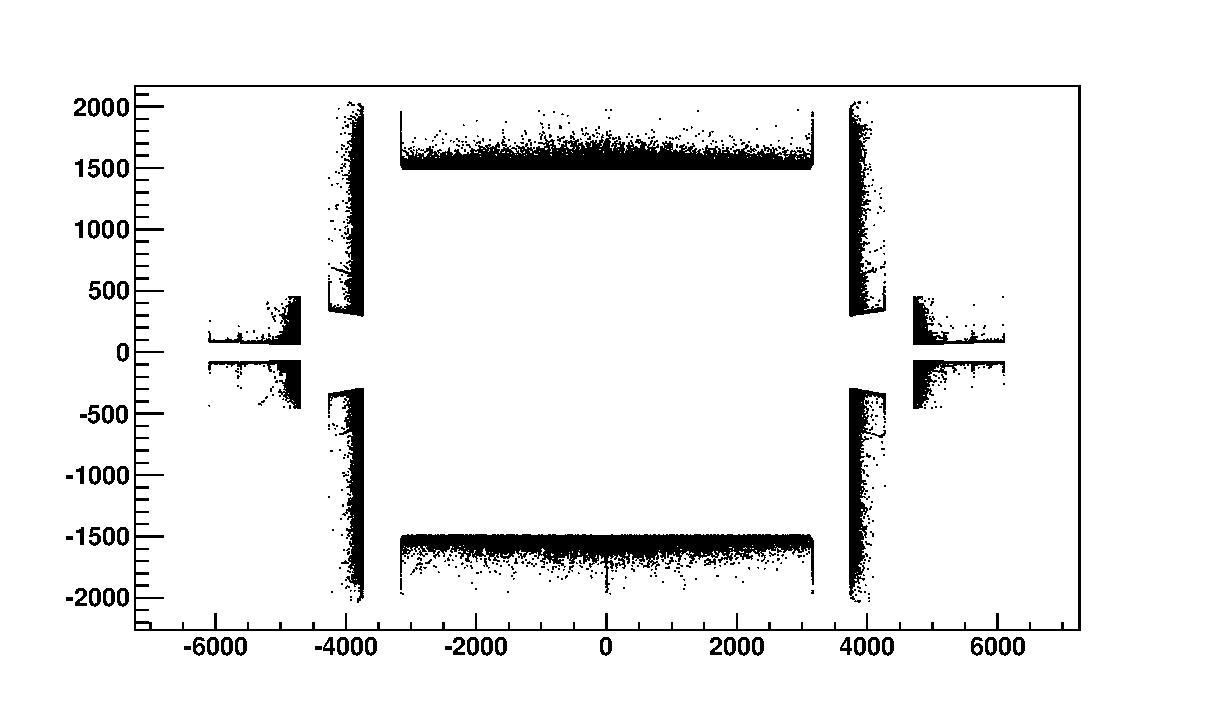
\includegraphics[width=1.0\textwidth]{figures/MC_FS_stpoints.eps}
\caption{The first stage of the 2-staged library production: FS starting point generation}
\label{fig:MC_FS_stpoints}}
\end{figure}

\begin{figure}[htb]
\center{
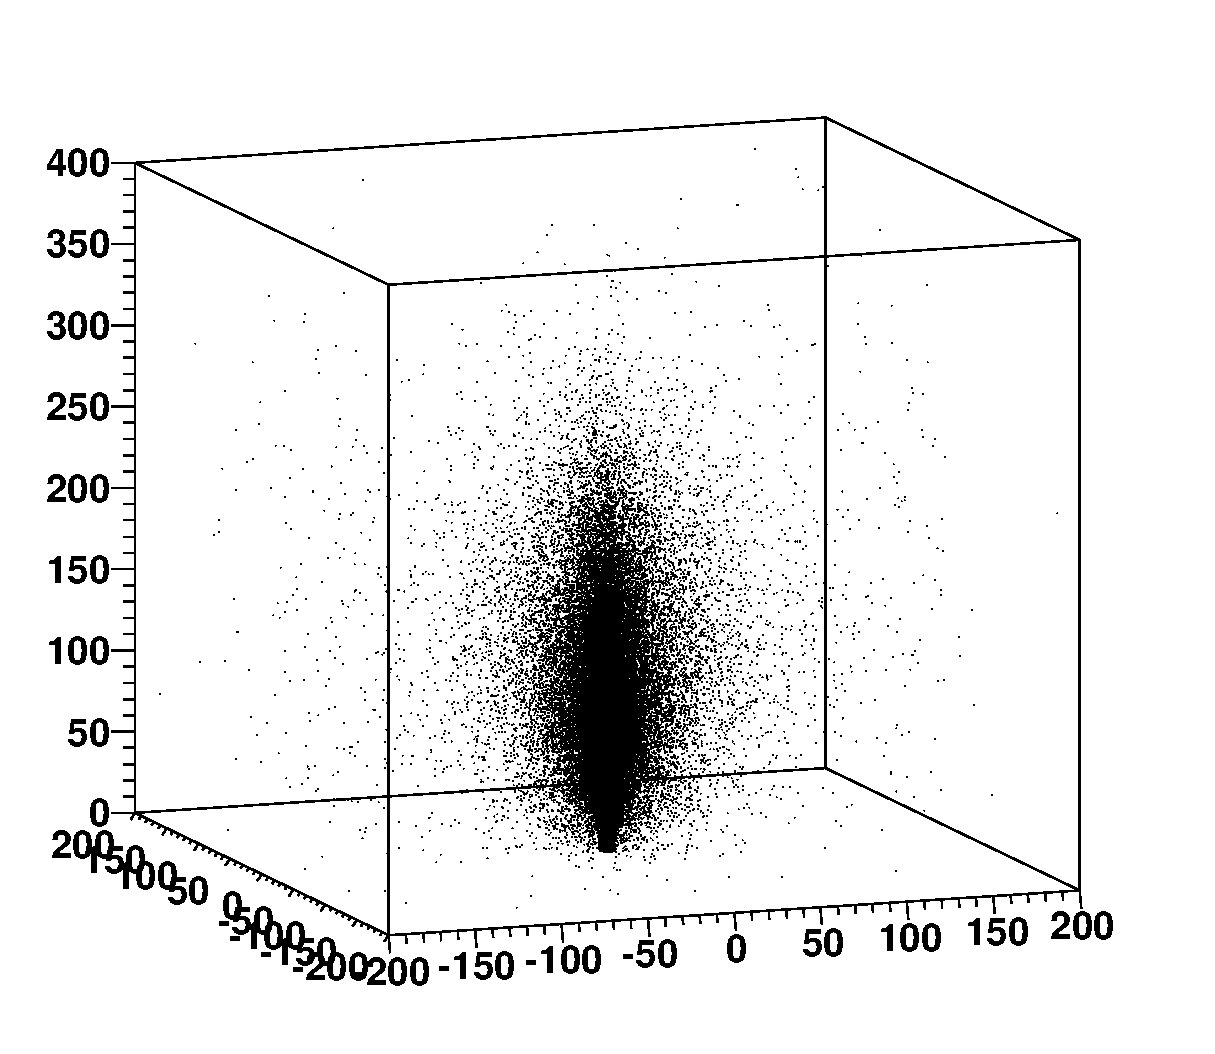
\includegraphics[width=0.75\textwidth]{figures/MC_FS_shower.eps}
\caption{The second stage of the 2-staged library production: the simulation of the shower}
\label{fig:MC_FS_shower}}
\end{figure}

This way of library generation solves all the problems mentioned above. The bin population problem does not occur because we produce the showers based on the real MC samples, and the resulting size of each kinematic bin is in direct dependence of the number of times this bin is used. This allows to reduce the size of the library and yet make a bigger diversity.

The post-processing stage consists of merging of the adjacent hits and of removing the far-standing hits that won't contribute to the reconstructed cluster anyway. Also, during this stage the size of the shower is calculated. It is used for containment check during the production.

The tuning of the library can then be applied manually in order to make the results the FS simulation closer to full simulation or the data. As this is a process that can't be (as of yet) done automatically, it requires lots of time and effort.

\subsubsection{FS production use}
\label{sec:MC_FS_prod}

During the production run the simulation software checks constantly if any particle agree with the parameterization criteria, which is the energy range (should be low enough) and the sub-detector containment (the particle should be far enough from the edges of the sub-detector volume for shower to fit within). The containment check is energy-dependent, because the sizes of the showers grow with energy, and the more energetic particles should be further from the edges in order for shower to fit.

When the particle with the proper parameters is found, it is then removed from the simulation and replaced with the shower. Before the deposition, the shower is scaled to fully correspond to the particle in energy.

\begin{figure}[htb]
\center{

\includegraphics[width=1.0\textwidth]{figures/blank.eps}
\caption{The simulation speed-up in case of single electron simulation for energy range $100-200 GeV$}
\label{fig:MC_FS_speedup}}
\end{figure}

For the MC11b campaign, the data from which is used in this analysis, frozen showers system was enabled by default in FCAL. Several studies showed that the errors introduced by the FS is negligible compared to the errors between MC and data, while the simulation speedup was about 25\%. The smallness of the errors introduced by the FS compared to other fast simulation methods (most notably - FastCaloSim) leaded to the misunderstanding, when the simulation with the FS system enabled was called "full simulation" as opposed to other, less precise but faster methods, which were called "fast simulation". In this terminology, all of the MC samples used in this analysis are full simulations.

\section{MC samples used in analysis}
\label{sec:MC_periods}

\section{Something on reweighting and such}
\label{sec:MC_correction}

Zvtx + pileup

plots before \& after (MC/Data)
